\chapter{The MBTI (Erik)}

\begin{authors}
	Erik Hoy
\end{authors}

\noindent\rule{\linewidth}{1pt}

\begin{quotation}
One of the largest complaints I hear about the MBTI is that it puts people in boxes. What people fail to recall is that a psychological indicator is only as good as its interpretation- if you feel put in a box by the MBTI, its because you put yourself there. The MBTI points out where we are unique among our type; for example, how an INFP can be atypical and still be an INFP. We can and do experience all the axes of the Meyers-Briggs- the indicator simply notes preferences. So, instead of seeing it as a box, let it be a window- to freer expression, broader understanding, and a higher sense of the complexities of human life.
\begin{flushright}
	James Rushing, INFP (1998)
\end{flushright}
\end{quotation}

\noindent\rule{\linewidth}{1pt}

\begin{quotation}
\begin{center}
	What is the MBTI all about?
\end{center}
It helped me to understand that yes, other people are different from me. Have you ever said, "We just seemed to be talking on different wavelengths. I just didn't seem to be getting it though"? It was probably true. Everyone's brain is different and every personality is different. Have you ever had a disagreement because you and the other person were interpreting things differently? The MBTI is a good place to begin when trying to understand where the miscommunication was. Understanding the model helps you to communicate better with all types of people out there. And then you start to learn the intricacies of each type and find out that no person within a type is exactly like anyone else. Everyone lives in a unique way. Another important fact that the MBTI clarifies is that all these interpretations are important. If they were all INTJs (it pains me to say this), they would miss some important viewpoints. You need diversity and different opinions. Everyone is special and everyone is valuable. What all of the different types contribute to life makes the world all that much more beautiful and wonderful to live in.
\begin{flushright}
	Heather Bailey, INTJ (1999)
\end{flushright}
\end{quotation}

\noindent\rule{\linewidth}{1pt}

\section{Letters}

The Meyers Briggs Type Indicator (MBTI) rates a person on four separate axes based on their personal preferences on each axis. Each axis has two parts which represent the two different outlooks and preferences common to each axis. 
The first axis describes one's attitude toward the world. This could also be seen as where a person likes to focus their mind and energies. The two attitudes are called introversion and extroversion. An introvert is one who is focused internally. Introverts are often quiet and reserved keeping their energy inside themselves. Extroverts, on the other hand, release this energy into the world.  They are often personable people and favor outer rather than inner expression. They may be called outgoing, friendly, loud, or exciting while introverts tend to fit descriptions such as reserved, shy, or solitary. Generally speaking, an introvert would rather join a few friends for a quiet game than go to a large party as many extroverts would. As will be discussed later, this first axis plays a major role in the way one interacts with the world. One's dominant function (Intuitive, Sensing, Thinking, or Feeling) is always in line with the person's attitude. In other words, if a person is extroverted/introverted their dominant function will be too. More on this later.
To understand the world, one must see it. That is the idea behind the second axis, perception. This axis describes how one perceives the world around them. This can be one of the most devise axis is as it represents two different systems of seeing the world. One side of the axis is that of sensing. The other is intuition. A sensing person relies on their senses to perceive the world around them. Such a person tends to be materially based and often highly factual. Sensing people tend to like hard facts and data, and often have to "see it to believe it." They generally tend to be good with details and often have precise memories. Their counterparts, the Intuitives, are based not on facts but on imagination and ideas. They rely on their intuition to perceive the world usually through dreams, ideas, thoughts, feelings, or visions. Theory and the abstract have much appeal to Intuitives, and they often value creativity. While Sensing types tend to work logically and practically toward a goal, Intuitives rely on bursts of insight and creativity often jumping from idea to idea to reach their "goal." They will "read between the lines" and tend to look for creative ways to solve a problem.
Once one has perceived the world, one has the option to judge it. That is what the third axis is for. It is the judgment axis with its two parts, Thinking and Feeling that is used to make decisions about the information that one absorbs. A Thinker is generally a logic based person who uses logic and reason to uncover the "truth" of a situation. For that matter, truth is often highly prized by Thinkers. Thinkers tend to seek truth in a logical and impersonal matter as if trying to find gold in dirt. Fairness is often highly important to thinkers who don't want their feelings to get in the way of making a judgment. Their counterparts, the Feelers, are at odds with these as they use their personal feelings and beliefs to make their decisions. They are focused on people rather than truth and often look for solutions that are best for the people involved rather than the most "truthful" ones. They tend to compromise rather than "seek the truth" in a conflict situation. Whereas thinkers often seen as direct or sometimes untactful, Feelers tend to be indirect and tactful as they are concerned with the feelings of others.

The final axis describes one's orientation toward the outside world. The two sides of this axis are Judging and Perceiving. Judging people tend to be goal focused and like order and direction. They are often planners and organizers who like to make lists and organize what interests them. They often prefer to act and make decisions rather than wait and respond. Perceiving people, on the other hand, prefer to remain more open and flexible. They often dislike organizing and prefer to "go with the flow" of life. They are often more scattered than their Judging counterparts but are more flexible and adaptable.  Neither function is exactly true to its namesake. Being a Judger or Perceiver does not mean that one is judgmental or perceptive. It is simply one's favored way of reacting to the outside world.

	Each axis is part of the four letter combination that makes a Meyers-Briggs type. One preference from each axis is chosen in order (attitude, perception, judgment, and orientation) based on the person's test results. These preferences are shortened to the letters E, I, S, N, T, F, J, and P to create one's type. The types created are as follows. (See Chart A)
	
However there is more to it than just one's type. Each type has four primary functions (MBTI letters) which are used to interact with the world. These four functions are the Sensing, Intuition, Thinking and Perceiving traits which are ranked according to the dominance of the trait and when it was developed. The middle two letters of one's Meyers-Briggs type are major functions which are developed early in life and are generally dominant. (Example- An INFJ would have N and F as the major (dominant and auxiliary functions) The opposite two letters are the minor functions which are developed later in life and are generally weaker than the major functions. The dominant function, as discussed earlier, is the primary trait/function one uses in everyday. It is in line with the attitude axis. It is either Introverted or Extroverted depending on which the person mode of interaction prefers overall (one's type on that axis). It is the function that one develops first and usually becomes the most adept with. A person usually prefers this function throughout their life and is comfortable using it.

	The dominant function is supplemented by the auxiliary function which similar to the dominant one is a comfortable one to use and a favored function for use in everyday life. It is developed after the dominant function and acts as a supplement to it. The introversion/extroversion preferences of the auxiliary function are the opposite of one's Meyers-Briggs type. For example, the auxiliary function of an INTP would be extroverted intuition with inverted thinking as the dominant function. These functions tend to work together to shape a person's worldview and decisions. They are usually the preferred functions throughout a person's life.
	
	The two functions not present in the person's MBTI type (minor functions) become the tertiary and inferior functions. These functions are weaker than the other two and develop later. They require effort to develop and rarely do so until later in life. They can be developed at anytime, but using them often requires a fair amount of initial discomfort. They are much like a person's non-dominant hand. One can use them effectively, but only with effort. These functions parallel the major functions in the sense that the weakest function (inferior) is the opposite of one's dominant function while the second weakest (tertiary) is the opposite of one's auxiliary function. (See Chart B)
	
Just to note, the results of the MBTI are not set in stone. Results can and do change over multiple taking of the test. The nature of the change is currently under debate. The two ideas have come to the fore. One is that type is fixed and one has only one "true" type. The change is simply that one had a false test due to bad questions or social/family/ etc. pressures and not due to a real change between the tests. The other is that type can change over the course of one's life. In practice, the effect is similar. The results one has now may not apply ten years from now. There are even type mistakes/switches that are common enough in the United States to have their own names. The primary one is called a Thinker mask. It is when a Feeler tries to act like a Thinker to "fit in" with society. It is especially common among young males. Social choices such as this one can lead to false results on the test. It is advisable to look into a type to make sure it fits before accepting it as "your type." If it does not fit, a retest may be in order. The general stereotype for a U.S. male is probably ESTJ. For a female it is ISFP. Those in U.S. society who do not fit these stereotypes (INFP males and ENTJ females for example) are likely to have a harder time "fitting in" to society and may feel out of place or inferior however one's type is nothing to be ashamed of. It has been found that there is little real connection between personality type and gender. For example, around half of men are feelers and half are thinkers. The same applies to women as well.  So not fitting the stereotype is actually quite a common phenomenon even on only one axis and is not something to be ashamed of. 

\section{Applications}

In Mentor, the MBTI takes a new form not seen in many other places. It becomes a language of understanding. "I'm an I and you're an E, and that's ok. We may not see eye to eye, but we both have gifts to share." The types are intended to validate and uplift, not label and tear down. When a Mentor student says, "I'm an INTP" they mean more than just the label. He means that is his preference. It is a shorthand way of saying, "I'm a person who prefers to use logic and intuition to work on internal ideas and issues$\ldots$" INTP is really a vague summery not a definite description. In mentor, the summery is used to make it easier to understand ourselves and others by giving each student a rough profile of himself with which he can relate with others of different types more easily. In general, this leads to greater interpersonal understanding and acceptance.

This is especially clear during shadow work. The shadow is in MBTI sense the personal opposite, all of the non-dominant letters. For an ESTP, his shadow would be the INFJ. The MBTI shadow is an excellent way to see what preferences one might have that one is not developing. Bringing these preferences out of the shadow can definitely enhance one's life. Having access to all preferences at will is extremely empowering as it allows one to flow with the situation. At ease with oneself, one can choose the best way to respond rather than acting sticking with preferences to a fault. Using logic in the place of love just won't cut it in a relationship, and those math problems can't be solved by crying.

To note, the Meyer-Briggs type indicator is considered to be a "fluffy" test and not up the standards of other, more professional personality tests. It is not an absolute determiner of type and is only a helpful indicator of one's likely personality and preferences which assists one in understanding oneself. It does not tell anyone how to behave. In fact, it is possible to differ significantly from the "average" personality of a particular type and still test as that type albeit with low and possibility inconclusive scores on one or more axis. In fact, strength or weakness on a particular axis (noted by scores usually between 1 and 60 on the test) can greatly alter the final result and produces an even wider range of results. An INTJ with very high scores in all categories is highly to be very different than an INTJ who scores less than 10 points toward each of their preferred axis's. This would also technique change their type to XXXX as a score less than 10 is considered to be too close to be at least moderately certain of its accuracy.

In short, while the MBTI is an extremely helpful tool for self-discovery and interpersonal communication, it is not something to be used as a professional test or a way to win arguments because "a fancy test said so." It is also worth noting that businesses can not use one's MBTI type as a pretext to refuse an application or tell the applicant that he or she is not able to do the job. It also does not say that one can on the basis of one's type. It is not something one should base one's life decisions on. As the next section will show, theory itself has its own points of contention.

\section{Type vs. Temperament}

Within the MBTI supporters there are generally two camps, type theorists and temperament theorists. Temperament theorists, led by Dr. David Keirsey, argue that people are born with one of four temperaments Keirsey labeled as Dionysian, Promethean, Epimethean, and Apollonian and then settled into one of the sixteen types later in life. In his view, one's type is fairly set and static once developed and the best thing one can do is develop his or her traits to the fullest. For example, an Intuitive should not bother with Sensing traits and should instead focus on developing Intuitive traits to their maximum potential. For more information about his theories, Please Understand Me I \& II by Keirsey are good reads for those who have a good knowledge of the MBTI and seek to dig into the theory a little deeper. For those who wish though take note for there is another theory to look at, type theorists. 

The type theorists are generally followers of Jung. They argue that insufficient evidence is available to prove that type is genetics and that the ideal is not just to develop one's favored traits but to develop all traits to their fullest with a mind toward balance. One can use any trait when it is appropriate. According to type theorists, people use all the type each day but out of habit or force of mind fall into comfortable preferences. They also assert that there are me dimensions to personality than the MBTI can show and can affect one's behavior in ways that the test can not predict. For further reading on this theory, Looking at Type: The Fundamentals would be a good place to start.

\section{Examples/Interviews/Challenges}

\subsection{Example of MBTI as a Shorthand}

\begin{quotation}
Try losing an argument? Even if you really believe your point? This practice has helped me tremendously. This is especially useful if you ever date an F. ;) Often it has been my experience that T's dominate arguments at all costs and F's can leave feeling low. The T can be derisive because the F isn't speaking the "proper" language of logic. Oh, now I've never been guilty of this, but everyone around me has. ;) What good is it always being right? No fun. So I try, against all friction, to shut up and say, "You know, that's a good point I hadn't thought of. You may be right, there." If you're in a relationship and the balance of argument winning is off, there'll be a lopsidedness to the relationship. I stripped away a girl's self-esteem after 2 years of this. I don't think she ever "won" the argument. This is the F way of thinking about it, I think. I cared about her so I've rethought how to deal with arguments. The T way would be to look at the situation, and see that you obviously aren't getting at the truth. 'Nuff said.

Thanks for writing. Your insight here is right on! \\
Love, \\
Q \\
\begin{flushright}
	Quinton Westrich, INTP (6-30-07)
\end{flushright}
\end{quotation}

\subsection{Excerpts from Journals: Examples of different types and how they think}

\begin{quotation}
This whole thing led me to the conclusion that I was not as open with others as I had thought I had been. If it was difficult to share with all of you before, it is much easier now. I am not completely reconciled with all above conclusions, but I am confident in the truth found in the journey.
\begin{flushright}
	Craig Schuff, INTP (3-2-04)
\end{flushright}
\end{quotation}

\noindent\rule{\linewidth}{1pt}

\begin{quotation}
 I've been getting really stressed this week trying to get things done. I'm not sure how so much started piling up, but Monday I made a list of everything I had to do (short and long term, so I don't forget) and I ended up with a typed page about 3/4 full (Ariel, size 10 font, for those interested). One of the big things is that I never finished putting everything away after the Chattcon (that journal will be out shortly) and my room had already been getting cluttered.
\begin{flushright}
	Shawn Trivette, ESTJ (1-31-02)
\end{flushright}
\end{quotation}

\noindent\rule{\linewidth}{1pt}

\begin{quotation}
	I felt if I could not earn friendship, I would earn respect from my peers. I always had to be the best at whatever I did. If I realized that I could not excel at something, I would not attempt it. While my childhood friends spent time playing basketball or baseball, I was reading and playing chess.
\begin{flushright}
	Mark Orr, INTJ (Fall 1996)
\end{flushright}
\end{quotation}

\noindent\rule{\linewidth}{1pt}

\begin{quotation}
	Is the framework EVER large enough, though? Once you push the boundaries out, and fill in the space, you push out some more$\ldots$ sigh. Life is pain. I understand that now, I really do. It's not a complaint, just an observation, sort of a constant that the Buddha observed on his path.
\begin{flushright}
	James Rushing, INFP (7-3-94)
\end{flushright}
\end{quotation}

\noindent\rule{\linewidth}{1pt}

\section{Quotes}

\section{Works Cited}

\section{Further Reading}

The choice of material in this chapter has heavily relied on that in \cite{Prov:87,MBTI:HHB:06,MBTI:HHB:02,Mar:95}.

Include a semi-annotated bib for each of the remaining books in the bib.

Chart A (new page)

Chart B (new page)

\begin{figure*}[htb]
		\scalebox{0.9}{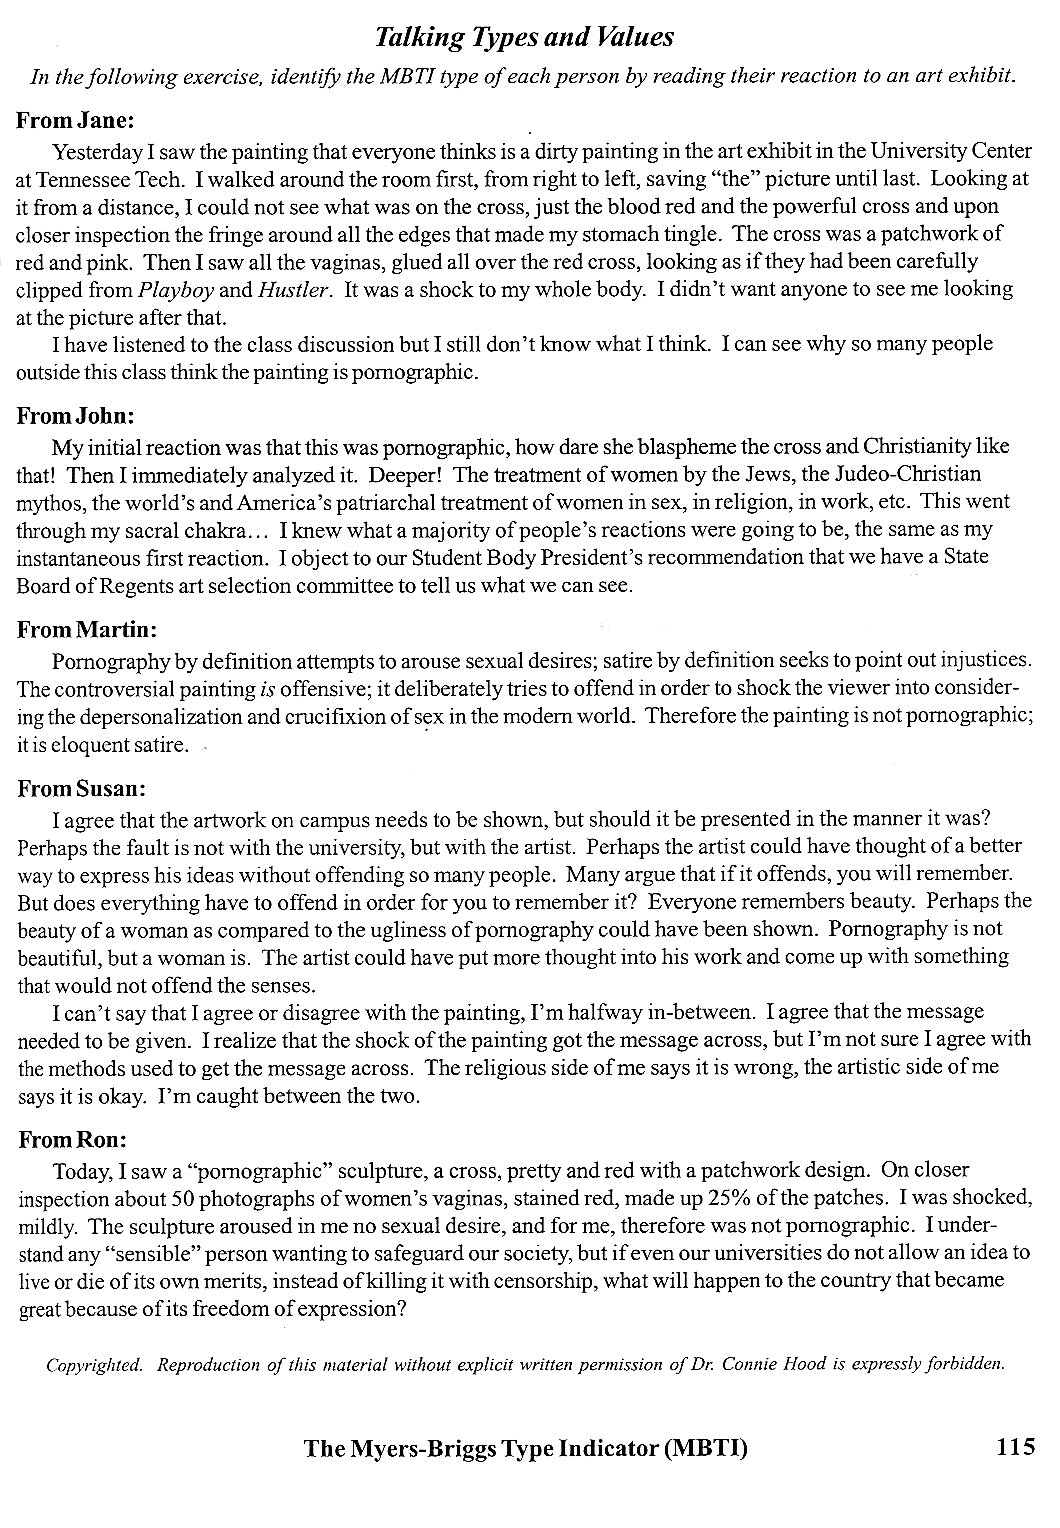
\includegraphics{mbti_test.jpg}}
\end{figure*}

\begin{figure*}[htb]
		\scalebox{0.9}{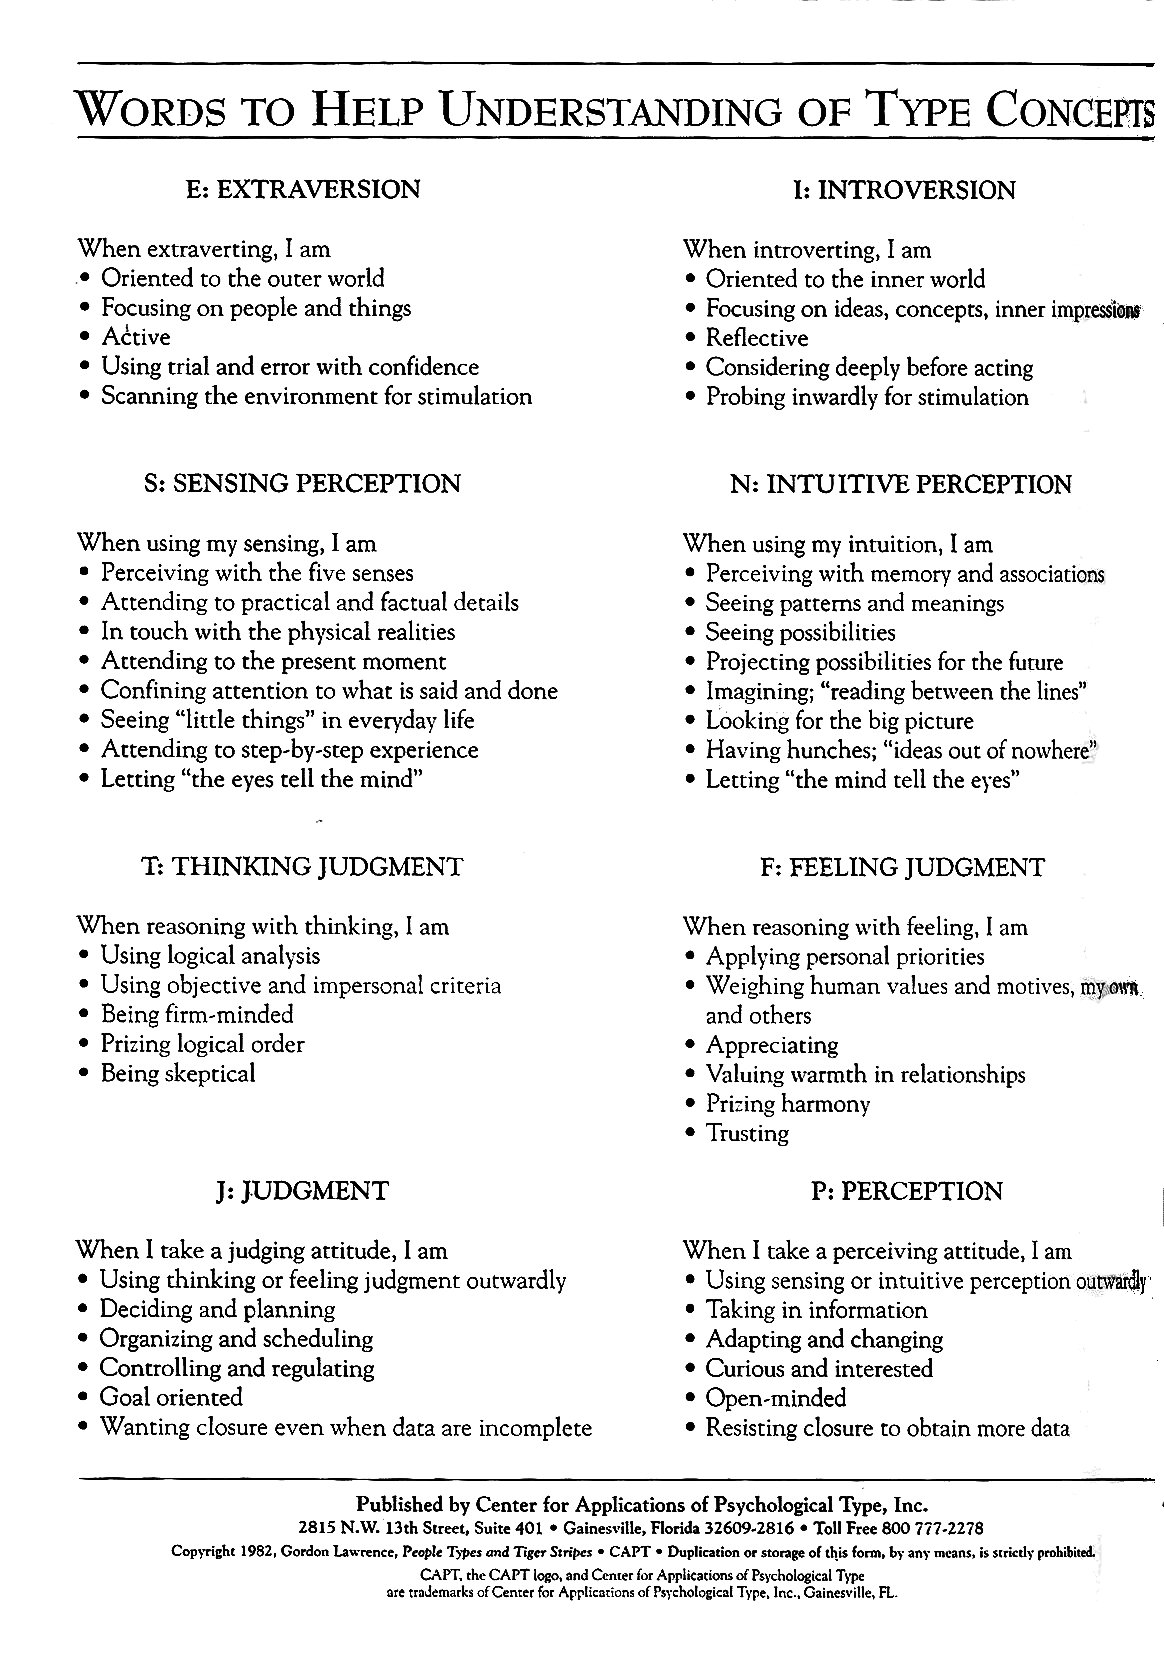
\includegraphics{understanding_type_concepts.jpg}}
\end{figure*}

\begin{figure*}[htb]
		\scalebox{0.8}{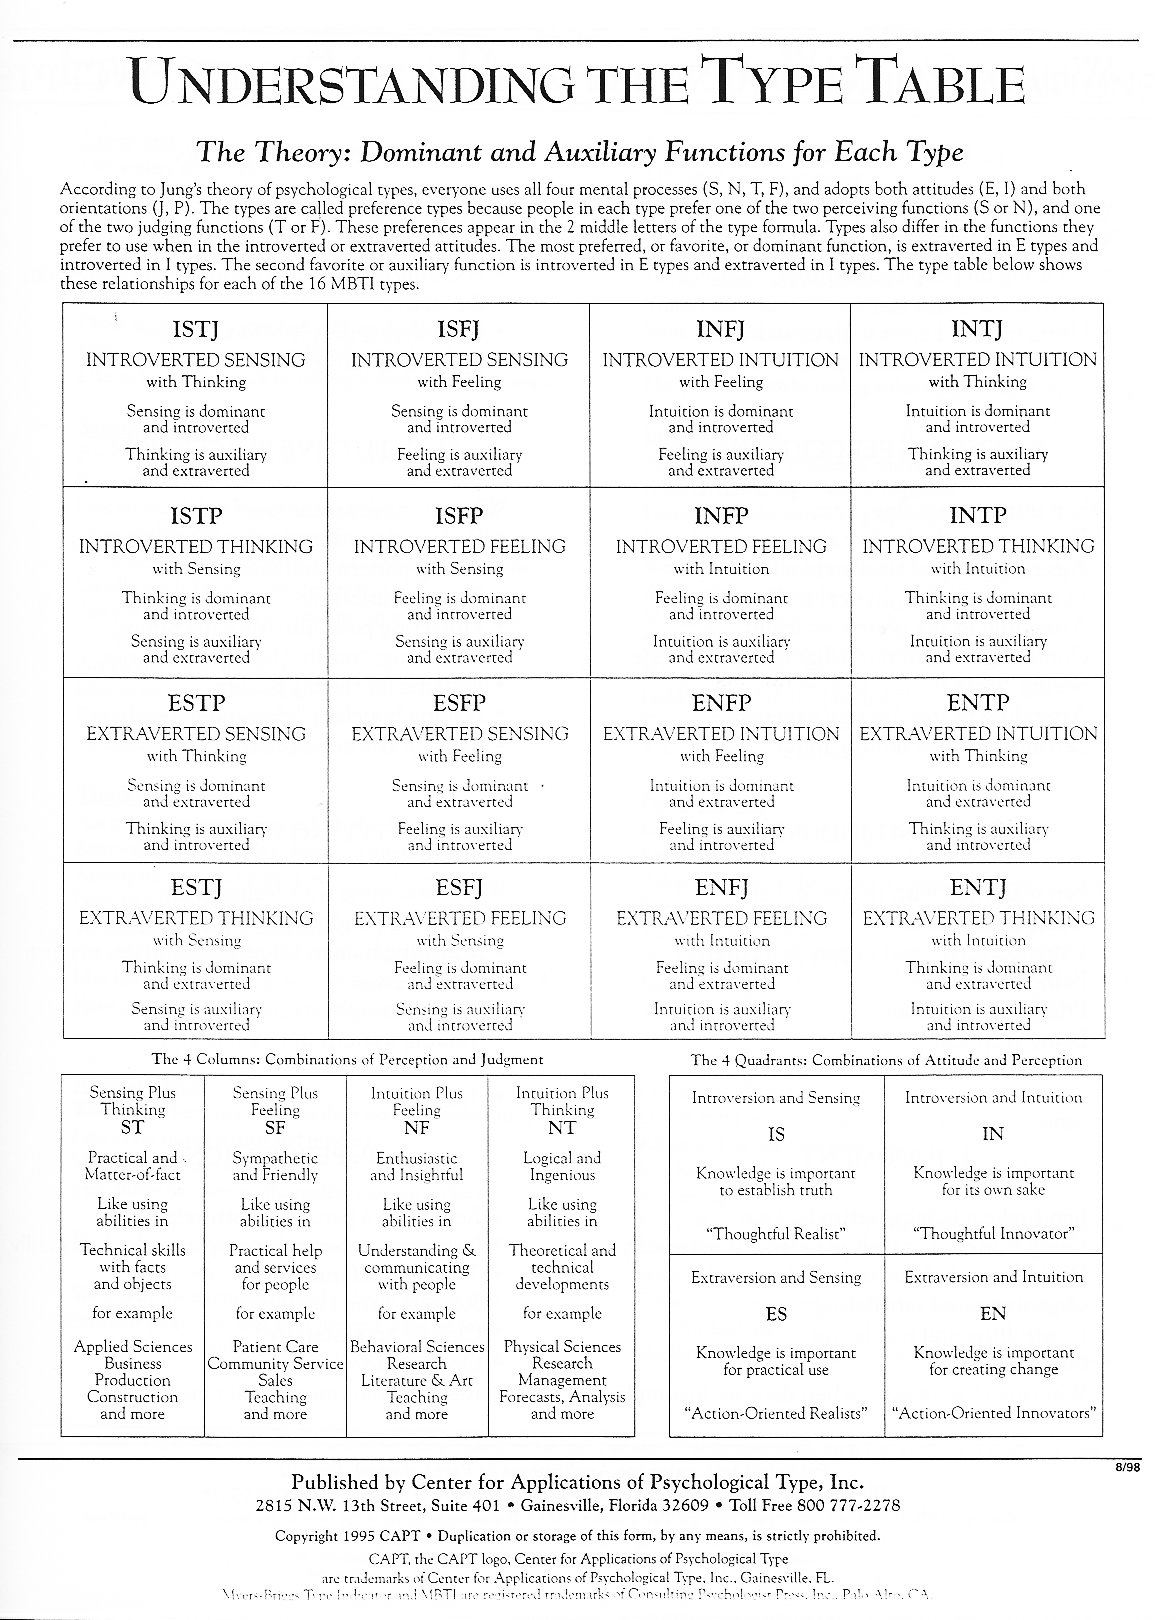
\includegraphics{understanding_type_table.jpg}}
\end{figure*}

\nocite{MBTI:HHB:06,Prov:87,Temp:86,Mar:95,MBTI:HHB:02,chood:87,Jen:95,Kei:98,Law:97,Mic:84,Mye:80}

\bibliographystyle{mla}		% the style you want to use for references.
\bibliography{mr,refs}				% the files containing all the articles and books you ever referenced.
